\PassOptionsToPackage{svgnames}{xcolor}
\documentclass[12pt]{article}



\usepackage[margin=1in]{geometry}  
\usepackage{graphicx}             
\usepackage{amsmath}              
\usepackage{amsfonts}              
\usepackage{framed}   
\usepackage{mathtools}            
\usepackage{amssymb}
\usepackage{array}
\usepackage{amsthm}
\usepackage[nottoc]{tocbibind}
\usepackage{bm}
\usepackage{enumitem}
\usepackage{ulem}

\DeclareMathOperator{\sech}{sech}
\DeclareMathOperator{\Tr}{Tr}
 \newcommand{\im}{\mathrm{i}}
  \newcommand{\diff}{\mathrm{d}}
  \newcommand{\col}{\mathrm{Col}}
  \newcommand{\row}{\mathrm{R}}
  \newcommand{\kerne}{\mathrm{Ker}}
  \newcommand{\nul}{\mathrm{Null}}
  \newcommand{\nullity}{\mathrm{nullity}}
  \newcommand{\rank}{\mathrm{rank}}
  \newcommand{\Hom}{\mathrm{Hom}}
  \newcommand{\id}{\mathrm{id}}
  \newcommand{\ima}{\mathrm{Im}}
  \newcommand{\lcm}{\mathrm{lcm}}
  \newcommand{\diag}{\mathrm{diag}}
  \newcommand{\inv}{^{-1}}
  \newcommand{\str}{^\ast}
  \newcommand\norm[1]{\left\lVert#1\right\rVert}
  \renewcommand{\labelenumii}{\roman{enumii}}
\setlength{\parindent}{0cm}
\setlength{\parskip}{0em}
\newcommand{\Lim}[1]{\raisebox{0.5ex}{\scalebox{0.8}{$\displaystyle \lim_{#1}\;$}}}
\newtheorem{definition}{Definition}[section]
\newtheorem{theorem}{Theorem}[section]
\newtheorem{notation}{Notation}[section]
\theoremstyle{definition}
\DeclareMathOperator{\arcsec}{arcsec}
\DeclareMathOperator{\arccot}{arccot}
\DeclareMathOperator{\arccsc}{arccsc}
\DeclareMathOperator{\spn}{Span}
\setcounter{tocdepth}{1}
\begin{document}

\title{ST2131/MA2216 AY1718 Sem 2 Answers}
\author{Lim Li}
\maketitle

\begin{enumerate}
\item 
\begin{enumerate}[label=(\alph*)]
\item
\[P(X=i) = pq^{i-1} = (1-q)q^{i-1} = q^{i-1} - q^i\]
\item
\begin{align*}
P(X \leq i) &= (q^0 - q^1) + (q^1 - q^2) + \cdots + (q^{i-1} - q^i) \\
    &= 1-q^i
\end{align*}
\item
\begin{align*}
P(W=w) &= P(w \leq F_Y^{-1}(U) < w+1) \\
    &= P(F_Y(w) \leq U < F_Y(w+1)) \\
    &= P(1-q^{w-1} \leq U < 1-q^w) \\
    &= q^{w-1} - q^w \\
    &= Geo(p)
\end{align*}
\item
\ \\
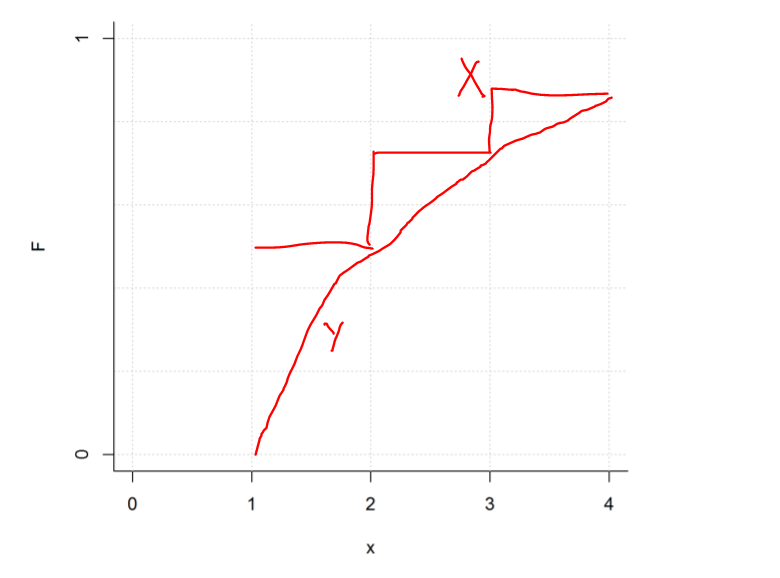
\includegraphics[scale=0.8]{graph.png}
\end{enumerate}
\item Let $C$ be the total sum of car weights
\[C \sim Z(115 \times 3, 115 \times 0.3^2)\]
\[W - C \sim Z(400 - 115 \times 3, 40^2 + 115 \times 0.3^2)\]
\begin{align*}
P(W < C) &= P(W - C < 0) \\
    &= P(Z < \frac{0-400 - 115 \times 3}{\sqrt{40^2 + 115 \times 0.3^2})} \\
    &= P(Z < -1.3706) \\
    &= 0.0852
\end{align*}
\item
\begin{enumerate}[label=(\alph*)]
\item
\begin{align*}
E(Y) &= \int_0^1 E(N(x,x^2)) \ dx \\
    &= \int_0^1 x \ dx \\
    &= \frac{1}{2} \\ \\
E(Y^2) &= \int_0^1 E(N(x,x^2)^2) \ dx \\
    &= \int_0^1 2x^2 \ dx \\
    &= \frac{2}{3} \\ \\
Var(Y) &= \frac{2}{3} - (\frac{1}{2})^2 \\
    &= \frac{5}{12} \\ \\
E(X) &= \frac{1}{2} \\ \\
E(XY) &= \int_0^1 E(XY|Y = x) \ dx \\
    &= \int_0^1 x^2 \ dx \\
    &= \frac{1}{3} \\ \\
cov(X,Y) &= \frac{1}{3} - (\frac{1}{2})(\frac{1}{2}) \\
    &= \frac{1}{12}
\end{align*}
\item
\[U = g(X,Y) = Y/X, V = h(X,Y) = X\]
\[x = v, y = uv\]
\[J(x,y) = \begin{vmatrix}
\frac{\partial g}{\partial x} & \frac{\partial g}{\partial y}\\
\frac{\partial h}{\partial x} & \frac{\partial h}{\partial y}
\end{vmatrix}
= \begin{vmatrix}
-\frac{y}{x^2} & \frac{1}{x} \\
1 & 0
\end{vmatrix}
= -\frac{1}{x}\]
\begin{align*}
f_{U,V}(u,v) &= f_{X,Y}(x,y) |-x| \\
    &= \frac{1}{\sqrt{2\pi}} \exp\{-\frac{1}{2x^2} (y-x)^2\} \\
    &= \frac{1}{\sqrt{2\pi}} \exp\{-\frac{1}{2v^2} (uv-v)^2\} \\
    &= \frac{1}{\sqrt{2\pi}} \exp\{-\frac{1}{2v^2} (u^2v^2-2uv^2+v^2)\} \\
    &= \frac{1}{\sqrt{2\pi}} \exp\{u - u^2/2 - 1/2\} \\
\end{align*}
Which is not even dependent on $v$. Hence, they are independent.
\end{enumerate}
\item
Note that $|Y| \sim Unif(0,1)$
\begin{align*}
P(Z < k) &= \int_0^1 P(X/y < k) \ dy \\
    &= \int_0^1 P(X < ky) \ dy
\end{align*}
If $0 < k < 2$, then $ky < 2$, hence, $P(X < ky) = ky/2$
\[P(Z < k) = \int_0^1 P(X < ky) \ dy = \int_0^1 ky/2 \ dy = k/4\]
\[\therefore f_Z(k) = 1/4\]
Else, if $k \geq 2$, then $2/k \leq 1$
\begin{align*}
P(Z < k) &= \int_0^1 P(X < ky) \ dy \\
    &= \int_0^{2/k} P(X < ky) \ dy + \int_{2/k}^1 P(X < ky) \ dy \\
    &= \int_0^{2/k} ky/2 \ dy + \int_{2/k}^1 1 \ dy \\
    &= (k/4)(2/k)^2 + (1-2/k) \\
    &= 1 - 1/k
\end{align*}
\[\therefore f_Z(k) = 1/k^2\]
\item
Define $R_0 := 0$

Suppose $E(R_i) = i$ for all $i=0,1,\cdots, n-1$. We want to show that $E(R_n) = n$ by induction. The base case of $i=0$ is trivial.

\begin{align*}
E(R_n) &= E(1 + \sum_{i=0}^n P(X_n = i)R_{n-i}) \\
    &= 1 + \sum_{i=0}^n P(X_n = i)E(R_{n-i}) \\
    &= 1 + \sum_{i=0}^n P(X_n = i)(n-i) + P(X_n = 0)(E(R_n) - n) \\
    &= 1 + n \sum_{i=0}^n P(X_n = i) - \sum_{i=0}^n i P(X_n = i) + P(X_n = 0)(E(R_n) - n) \\
    &= 1 + n (1) - E(X_n) + P(X_n = 0)(E(R_n) - n) \\
    &= 1 + n (1) - 1 + P(X_n = 0)(E(R_n) - n) \\
    &= n + P(X_n = 0)(E(R_n) - n) \\
\end{align*}
\[\therefore E(R_n) = n + P(X_n = 0)(E(R_n) - n)\]
\[\therefore E(R_n) = \frac{n - n P(X_n = 0)}{1 - P(X_n = 0)} = n\]
\end{enumerate}



\end{document}